\documentclass{beamer}
\usetheme{Darmstadt}
\AtBeginSection[]
{
\begin{frame}
    \frametitle{Presentation Outline}
    \tableofcontents[currentsection]
\end{frame}
}
\addtobeamertemplate{navigation symbols}{}
{
\hspace{1em}
\usebeamerfont{footline}%
\insertframenumber / \inserttotalframenumber
}
\setbeamertemplate{caption}[numbered]

\usepackage{graphicx}
\graphicspath{{./tikz/}{../report/}}
\usepackage{amsmath}
\usepackage{adjustbox}
\usepackage[style=phys, backend=biber]{biblatex}
\renewcommand*{\bibfont}{\scriptsize}
\addbibresource{ref.bib}
\nocite{*}
\usepackage{caption}
\captionsetup{font=scriptsize}
\usepackage{tcolorbox}
\usepackage{tikz}
\usetikzlibrary{shapes}
\usetikzlibrary{external}
\tikzexternalize

\title{The Worm Algorithm}
\subtitle{physics760: Computational Physics\\Final Project}
\author{Ajay S. Sakthivasan \and Dongjin Suh}
\institute{Universität Bonn}

\date{March 15, 2023}
\begin{document}

\begin{frame}
    \titlepage
\end{frame}

\begin{frame}
    \frametitle{Presentation Outline}
    \tableofcontents
\end{frame}

\section{Introduction}
\begin{frame}{Introduction}
    \begin{itemize}
        \item The Metropolis algorithm is a widely used Monte Carlo method for the Ising model.
        \item However we face the problem of critical slowing down.
        \item Prokof’ev and Svistunov proposed an alternative update algorithm called the Worm Algorithm (WA).
        \item WA preserves the local nature of the update step, but achieves a very small dynamical exponent.
    \end{itemize}
\end{frame}

\section{Theoretical Basis}
\subsection{The Ising model}

\begin{frame}{The Ising model}
\begin{itemize}
    \item A mathematical model to understand the behaviour of systems phase transitions, like ferromagnetic materials
    \item 2D Ising model: Magnetic system consisting of interacting spins on a two-dimensional lattice
\end{itemize}

Hamiltonian: 
    \begin{align*}
    H = J\sum_{\langle i,j \rangle} s_{i}s_{j} - h\sum_{i} s_{i}
\end{align*}

Partition function: 
\begin{align*}
    Z = \sum_{s} \mathrm{e}^{-\beta H} = \sum_{s} \mathrm{e}^{-[-\beta J \sum_{\langle i,j \rangle}s_i s_j - \beta h \sum_{i}s_i]}
\end{align*}
\end{frame}

\subsection{Physical observables}
\begin{frame}{Physical observables}
    Describe the properties of the system change at phase transition   
    \begin{itemize}
        \item Magnetisation per spin 
            \begin{align}
            M = \frac{1}{N}\sum_{i}^{N} \sigma_{i}
            \end{align}
            N replaced by $L^{2}$, where L is the lattice length and $\sigma$ the spin. \\
        \item Energy per site
            \begin{align}
            E = \frac{1}{N} H
            \end{align}
    \end{itemize}
\end{frame}

\begin{frame}
    \begin{itemize}
        \item Susceptibility
        \begin{align}
        \chi = (k_B \beta) \cdot (\langle M^2 \rangle-\langle M \rangle^2)
        \end{align}
        \item Specific heat
        \begin{align}
        C = (k_B \beta)^2 \cdot (\langle E^2 \rangle-\langle E \rangle^2) 
        \end{align}
        \item Autocorrelation time – Dynamical Exponent ($z$) \\
        \begin{align}
        \tau \approx L^z \text{ for large J and } \beta
        \end{align}
    \end{itemize}
\end{frame}


\section{Methodology}

\subsection{Metropolis-Hastings Algorithm}
\begin{frame}{Metropolis-Hastings Algorithm}
    \begin{itemize}
        \item This is a Monte Carlo simulation method. 
        \item Generate samples from a probability distribution.
        \item Iterative update of the system with the Accept-Reject method.
        \item Implement Metropolis-Hastings method.
        \begin{enumerate}
            \item Random configuration of an N × N lattice.
            \item  Flip the spin at the site.
            \item Calculate the energy cost $\Delta$E of the flip.
            \item The reject/accept step.
        \end{enumerate}
        \item Repeat these steps for desired number of times and measure the observables at every iteration.
    \end{itemize}
\end{frame}

\subsection{The Worm Algorithm}
\begin{frame}{The Worm Algorithm}
\begin{itemize}
    \item The worm algorithm is an alternative to the standard Metropolis algorithm.
    \item The original implementation by Prokof'ev and Svistunov is roughly as follows:
    \begin{enumerate}
        \item Start with an arbitrary lattice configuration (with no starting bonds between the sites).
        \item Select an arbitrary point as $i_1 = i_2$.
        \item Grow the worm:
        \begin{enumerate}
            \item When $i_1 \neq i_2$, choose to move $i_1$ and create or erase bond line between the sites.
            \item When $i_1 = i_2$, choose with probability $0.5$ to start with a new site or to move $i_1$.
            \item The acceptance probabilities of the moves are given by solutions to the balance equation.
            \item Collect statistics for various quantities and proceed to moving the worm.
        \end{enumerate}
        \item Repeat the steps desired number of times.
    \end{enumerate}
\end{itemize}
\end{frame}

\begin{frame}
\begin{itemize}
    \item There are many variations of the worm algorithm.
    \item Our first implementation of the worm algorithm is as follows:
    \begin{enumerate}
        \item Start with an arbitrary lattice configuration.\footnotemark
        \item Select an arbitrary point to create the worm.
        \item Grow the worm: \\
        \begin{enumerate}
            \item Choose a random direction to move.
            \item If the new point is of the same spin as the old point, add it to the worm with probability 1.
            \item If not, perform a Metropolis-like check. If a flip is favourable, flip and add
            \item This way, we create a worm with equal spins.
            \item Break when the worm head meets its tail or if a flip is no longer favourable.
        \end{enumerate}
        \item Measure the observables.
        \item Carry out the desired number of iterations, with a new worm every time.
    \end{enumerate}
    \item There are a few caveats.
\end{itemize}
\footnotetext[1]{We started with an ``almost" cold start.}
\end{frame}

\begin{frame}
\begin{itemize}
    \item Given below is a worm at an intermediate step of its growth.
    \item The lattice below is a small part of the total lattice.
\end{itemize}
\begin{figure}
    \centering
    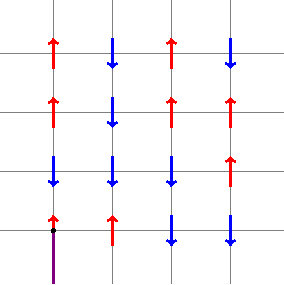
\includegraphics{tikz1.pdf}
\end{figure}
\end{frame}

\begin{frame}
\begin{itemize}
    \item The worm decides to move right.
    \item The new site has the same spin as the old site.
\end{itemize}
\begin{figure}
    \centering
    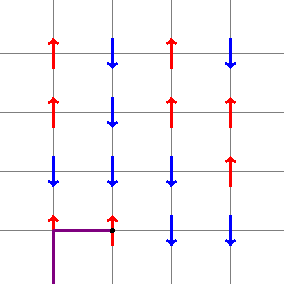
\includegraphics{tikz2.pdf}
\end{figure}
\end{frame}

\begin{frame}
\begin{itemize}
    \item The worm decides to move right.
    \item The new site has the opposite spin as the old site.
    \item Now we perform a metropolis-like check and decide whether to flip or not.
\end{itemize}
\begin{figure}
    \centering
    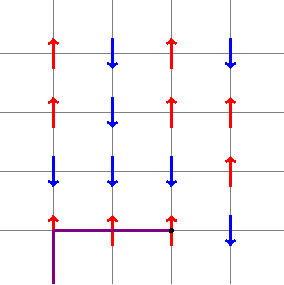
\includegraphics{tikz3.pdf}
\end{figure}
\end{frame}

\begin{frame}
\begin{itemize}
    \item The worm after a few more steps.
\end{itemize}
\begin{figure}
    \centering
    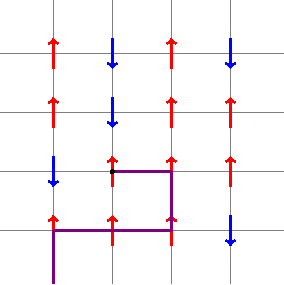
\includegraphics{tikz4.pdf}
\end{figure}
\end{frame}

\begin{frame}
\begin{itemize}
    \item Caveat: If the worm tries to move to a point that is already a part of the worm, we need to update the head accordingly.
    \item We want only an even number of bonds between the sites.
    \item We ensure this by choosing the new head and breaking an old bond appropriately (with equal probability).
\end{itemize}
\begin{columns}
\begin{column}{0.5\textwidth}
\begin{figure}
    \centering
    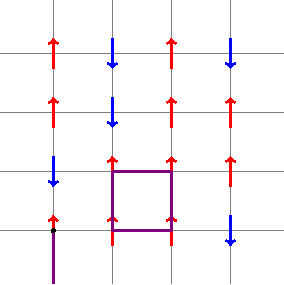
\includegraphics{tikz5.pdf}
\end{figure}
\end{column}
\begin{column}{0.5\textwidth}
\begin{figure}
    \centering
    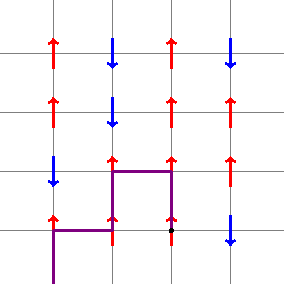
\includegraphics{tikz6.pdf}
\end{figure}
\end{column}
\end{columns}
\end{frame}

\begin{frame}
\begin{itemize}
    \item Caveat: If the worm tries to leave the lattice, let it choose a different direction.
    \item Caveat: The worm cannot be bigger than the total number of lattice sites.
    \item The worm dies if it hits its tail or if a new flip is no longer favourable.
    \item Update the observables and start with a new worm.
\end{itemize}
\end{frame}

\begin{frame}
\begin{itemize}
    \item \textbf{Problem}: This variation of the algorithm did not provide the expected behaviour at low inverse temperatures.
    \item \textbf{Reason}: Say we start with a random site. A flip is always favourable, and a worm keeps growing until breaking conditions are met.
    \item \textbf{Attempted Solution}: Try worms of alternating spins instead of same spins.
    \item This did solve the problem and resulted in the expected behaviour (including critical point).
    \item We also tried a mix of the two variations by introducing a cut-off.
\end{itemize}
\end{frame}

\begin{frame}{How does this differ?}
\begin{columns}
    \begin{column}[t]{0.5\textwidth}
    \begin{itemize}
        \item We always choose to kill the worm when the head and tail meet.
        \item We implemented a Metropolis-like check for acceptance probabilities.
        \item Observables are calculated from the lattice configuration at the end of a worm's life.
    \end{itemize}
    \end{column}
    \begin{column}[t]{0.5\textwidth}
    \begin{itemize}
        \item In the original implementation, this was done with a probability $0.5$.
        \item Acceptance probabilities are calculated based on the bond configuration.
        \item Observables are calculated directly from the bond configuration after every time the worm moves.
    \end{itemize}
    \end{column}
\end{columns}
\end{frame}

\subsection{Error Analysis}
\begin{frame}{Error Analysis}
\begin{itemize}
    \item Bootstrap method was used for error analysis.
    \item The idea is roughly as follows – we resample from the original sample to create multiple samples.
    \item For each sample, the statistic of interest is then studied.
    \item The standard deviation of the bootstrap distribution is an estimate of the standard error.
    \item This method was used to estimate the errors in the quantities in our results.
\end{itemize}
\end{frame}

\section{Results}
\subsection{Algorithm behaviour}
\begin{frame}{Algorithm behaviour – Metropolis}
    \begin{figure}[htbp]
	\begin{center}
		\begin{minipage}[t]{0.49\linewidth}
			\centering
			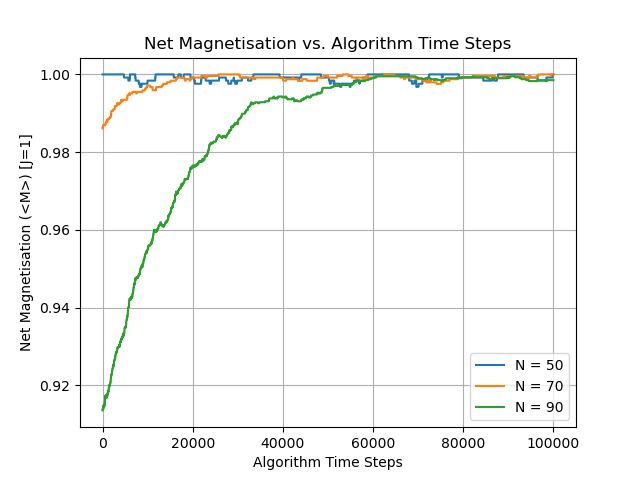
\includegraphics[width=\linewidth]{metro_algobehaviour1.png}
		\end{minipage}
		\begin{minipage}[t]{0.49\linewidth}
			\centering
			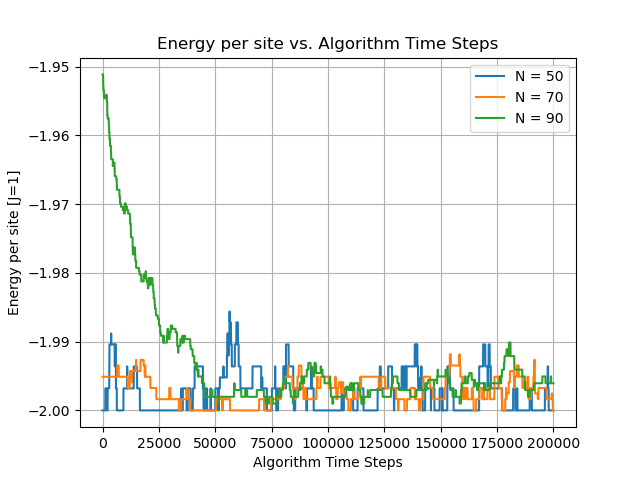
\includegraphics[width=\linewidth]{metro_algobehaviour2.png}
		\end{minipage}
        \caption{Metropolis behaviour studied with 100000 iterations of the algorithm with 30000 burn-in iterations, J = 1 and $\beta$ = 1}
	\end{center}
    \end{figure}
\end{frame}

\begin{frame}{Algorithm behaviour – Worm Algorithm}
    \begin{figure}[htbp]
		\begin{minipage}[t]{0.49\linewidth}
			\centering
			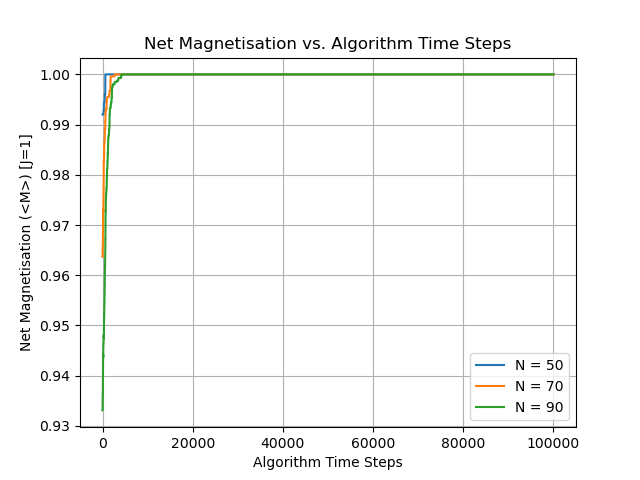
\includegraphics[width=\linewidth]{worm_algobehaviour1.png}
		\end{minipage}
		\begin{minipage}[t]{0.49\linewidth}
			\centering
			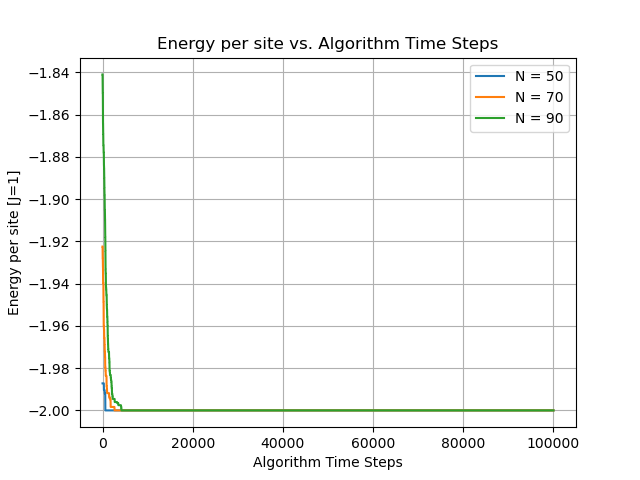
\includegraphics[width=\linewidth]{worm_algobehaviour2.png}
		\end{minipage}
    \caption{Worm behaviour studied with 100000 iterations of the algorithm with 30000 burn-in iterations, J = 1 and $\beta$ = 1}
    \end{figure}
\end{frame}

\begin{frame}
\begin{itemize}
    \item Both the cases were studied with the same initial configurations – ``almost'' cold starts closer to spins $= +1$ and $-1$ respectively.
    \item We immediately notice that the worm algorithm equilibrates much faster.
    \item Lattice size doesn't significantly affect equilibration in the case of WA.
\end{itemize}
\end{frame}

\subsection{Net Magnetisation}
\begin{frame}{Net Magnetisation}
    \begin{figure}[htbp]
	\begin{center}
		\begin{minipage}[t]{0.49\linewidth}
			\centering
			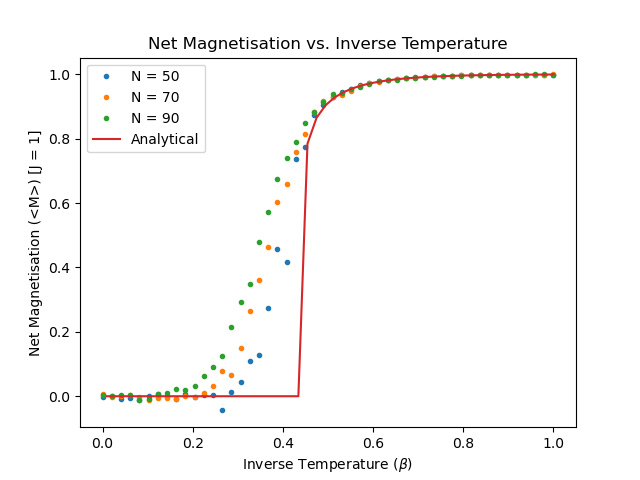
\includegraphics[width=\linewidth]{metro_netmag-beta.png}
            \caption{Metropolis algorithm: Behavior of net magnetisation}
		\end{minipage}
		\begin{minipage}[t]{0.49\linewidth}
			\centering
			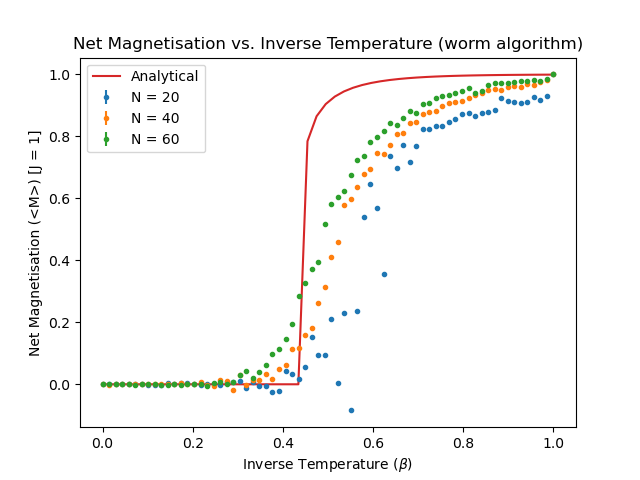
\includegraphics[width=\linewidth]{worm_netmag-beta.png}
		  \caption{Worm algorithm: Behavior of net magnetisation}
        \end{minipage}
	\end{center}
    \end{figure}
\end{frame}

\begin{frame}
\begin{itemize}
    \item WA was studied for smaller lattices – computationally more expensive when bootstrapping was included.
    \item We notice worm algorithm is much smoother around the critical points, even for smaller lattice sizes.
    \item However, it is a bit far from the analytical solution.
    \item As discussed, we experimented with two different implementations of worm algorithms – this plot corresponds to alternating spins.
    \item The other variation produced more exact result for high inverse temperature.
\end{itemize}
\end{frame}

\subsection{Susceptibility and Heat Capacity}
\begin{frame}{Susceptibility and Heat Capacity – Metropolis}
    \begin{figure}[htbp]
	\begin{center}
		\begin{minipage}[t]{0.49\linewidth}
			\centering
			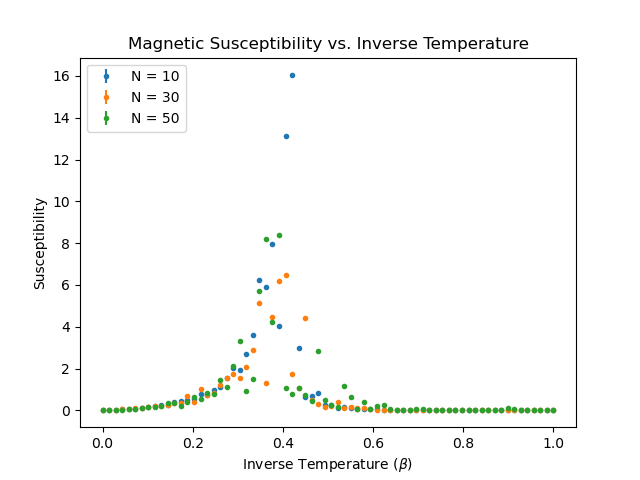
\includegraphics[width=\linewidth]{metro_chi-beta.png}
		\end{minipage}
		\begin{minipage}[t]{0.49\linewidth}
			\centering
			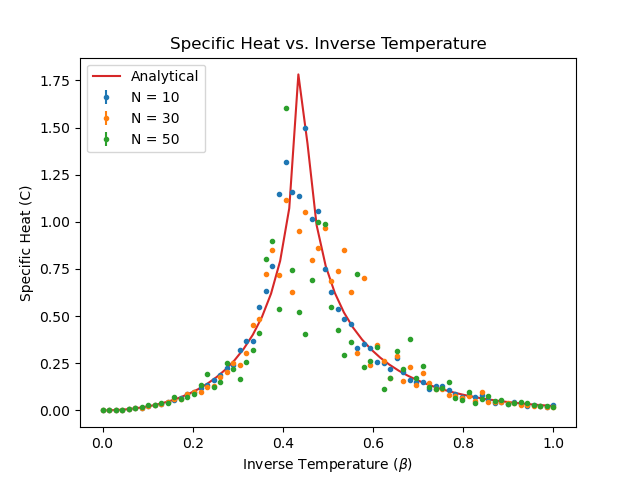
\includegraphics[width=\linewidth]{metro_c-beta.png}
		\end{minipage}
        \caption{Metropolis Algorithm: Behaviour of Susceptibility and Heat Capacity}
	\end{center}
    \end{figure}
\end{frame}
\begin{frame}{Susceptibility and Heat Capacity – Worm Algorithm}
    \begin{figure}[htbp]
	\begin{center}
		\begin{minipage}[t]{0.49\linewidth}
			\centering
			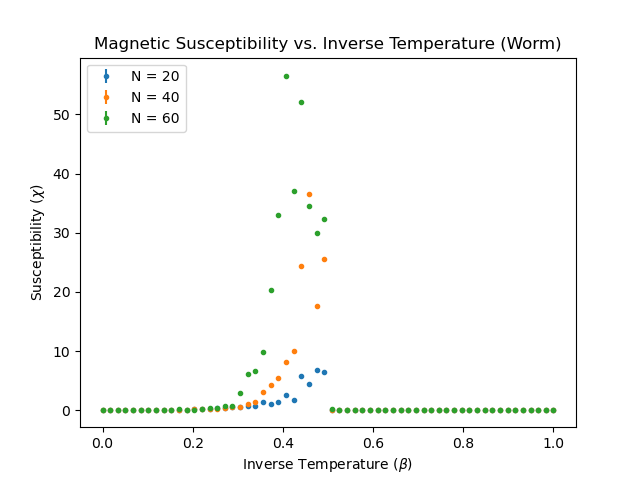
\includegraphics[width=\linewidth]{worm_suscep.png}
		\end{minipage}
		\begin{minipage}[t]{0.49\linewidth}
			\centering
			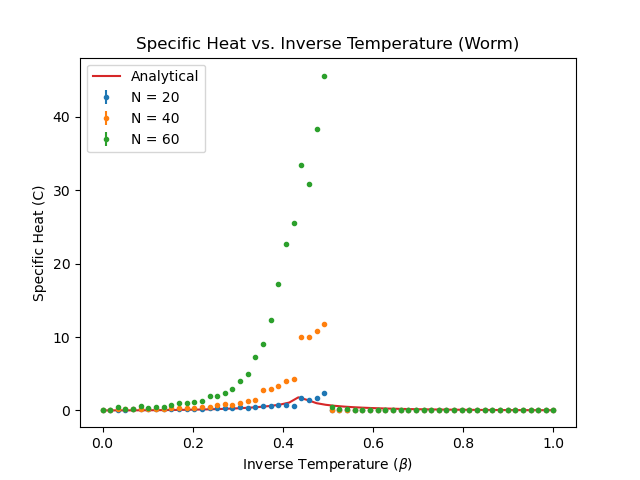
\includegraphics[width=\linewidth]{worm_heat_1.png}
		\end{minipage}
        \caption{Worm Algorithm: Behaviour of Susceptibility and Heat Capacity}
	\end{center}
    \end{figure}
\end{frame}

\begin{frame}
\begin{itemize}
    \item Again, the worm algorithm produced less sporadic points compared to Metropolis.
    \item However, we faced an issue with normalisation.
\end{itemize}
\end{frame}

\subsection{Autocorrelation time – Dynamical Exponent}
\begin{frame}{Autocorrelation time – Dynamical Critical Exponent}    
    \begin{figure}[htbp]
	\begin{center}
		\begin{minipage}[t]{0.49\linewidth}
			\centering
			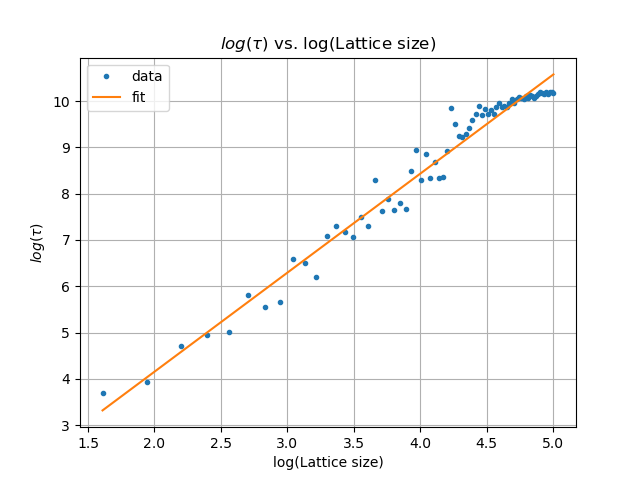
\includegraphics[width=\linewidth]{metro_dyncritexp.png}
		  \caption{Metropolis Algorithm: Behaviour of Autocorrelation Time}
        \end{minipage}
		\begin{minipage}[t]{0.49\linewidth}
			\centering
			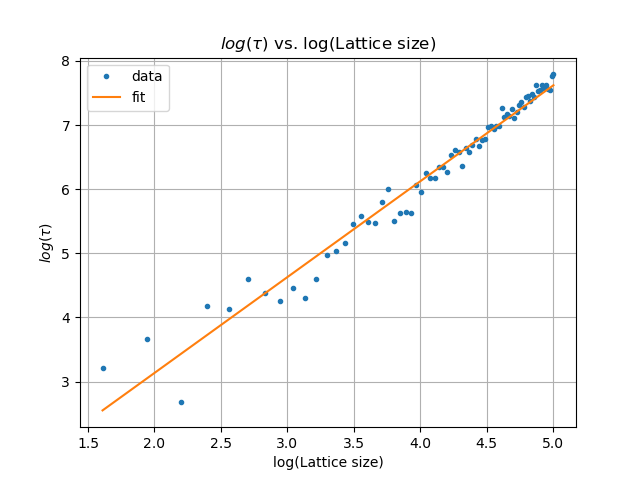
\includegraphics[width=\linewidth]{worm_dyncritexp.png}
		  \caption{Worm Algorithm: Behaviour of Autocorrelation Time}
        \end{minipage}
	\end{center}
    \end{figure}
\end{frame}

\begin{frame}
\begin{itemize}
    \item Lattice sizes from $5$ to $149$ were considered for autocorrelation times.
    \item The autocorrelation times were calculated, and then a $ln-ln$ plot was made.
    \item The plots here correspond to a dynamical critical exponent of $2.13$ and $1.49$ for Metropolis and WA, respectively.
    \item 20 different runs were carried out for autocorrelation time. Dynamical exponent had a range $2.1-2.21$ and $1.46-1.55$ for Metropolis and WA.
    \item Statistical analysis was not considered, since 20 runs are not enough.
\end{itemize}
\end{frame}

\section{Discussion}
\begin{frame}{Discussion}
\begin{itemize}
    \item The algorithm is functional to the extent that the results are not unreasonable.
    \item The dynamical critical exponent was reduced with WA, but still higher than the original work.
    \item In the original implementation, the dynamical exponent was reported as $0.25$.
    \item We believe this is mainly due to our decision to kill the worm and using a Metropolis-like check.
    \item However, this hypothesis needs to tested (maybe in the future).
    \item It should also be noted that lattice sizes up to $512$ were considered in the original work.
    \item Asymptotic result $\implies$ we might get a better result if we simulate larger lattices.
\end{itemize}
\end{frame}

\begin{frame}
\begin{itemize}
    \item When it comes to physical observables, the plots showed critical behaviour.
    \item However, they were not exact compared to analytic results.
    \item There is also an issue of normalisation, which, for some reason, proved to be very elusive in the case of WA.
    \item Primary goal for future work, replace with the variation in the original work.
    \item Measure observables using bond configurations.
    \item This should further improve our results.
    \item 3D Ising was not studied due to time constraints.
    \item Another course of work – Implement the algorithm for 3D Ising model.
\end{itemize}
\end{frame}

\section{Summary}
\begin{frame}{Summary}
\begin{itemize}
    \item To summarise, we studied the worm algorithm in this project.
    \item This was then used to simulate the 2D Ising model.
    \item Various observables and the dynamical critical exponent were calculated.
    \item The corresponding results were then compared with Metropolis algorithm.
    \item Shortcomings and problems with the implementation were realised, and possible solutions are suggested.
    \item Things that were left out due to time constraints could be studied in the near future.
\end{itemize}
\end{frame}

\begin{frame}
\centering
Thanks for your time!
\end{frame}

\begin{frame}[allowframebreaks]{References}
    \printbibliography
\end{frame}

\end{document}
